\documentclass{article}

% --- load packages ---

\usepackage[margin=1in]{geometry} % change the margins
\usepackage{amsmath} % useful math environments and commands like align
\usepackage{amssymb} % assumes amsmath package installed
\usepackage[colorlinks,bookmarks,bookmarksnumbered,allcolors=blue]{hyperref} % hyperlinks between references
\usepackage{graphicx}  % include images
\usepackage[caption=false]{subfig} % subfigures.  false option prevents conflicts in caption styling with other packages
\usepackage{booktabs} % better tables
\usepackage[capitalise]{cleveref} % better referencing. uses cref.
\usepackage[section]{placeins} % sometimes useful to prevent figures from floating out of a section
\usepackage{cite} % handles multiple citations in one command better
\usepackage{doi} % allow correct hypderlinking of DOIs
\usepackage{hyperref}
\usepackage{algorithm} % for algorithm figure
\usepackage[title]{appendix}
\usepackage{pgfplots}

\usepackage{aircraftshapes}

\newcommand{\norm}[1]{\left\Vert{#1}\right\Vert}
\newcommand{\skewm}[1]{\left[{#1}\right]_{\times}}


\begin{document}

\title{Homework 4}
\author{Jaron Ellingson}
% put in \date{} if you don't want a date to appear, or enter a specific date, otherwise default is today's date.
\maketitle

 %\href{https://byu.box.com/shared/static/anxheci3eytucrh3ke57k2sqdx0ivmjg.pdf}{homework pdf}

\section*{Introduction}

To explore constrained optimization, I choose to implement a simplified version of my final project. My project is to create a evolutionary nonlinear model predictive control for a fixed wing aircraft. We will simplify this problem by removing the evolutionary part and solving the nonlinear model predictive control (NMPC). It is important to note that usually model predictive control is preformed on linearized dynamics to allow for fast quadratic programming optimization. We want to explore solving nonlinear model predictive control which will not linearize the model and therefore is a little harder to solve.



\section*{Nonlinear Model Predictive Control}

The NMPC problem we want to solve is formulated by

\begin{equation*}
\begin{aligned}
\text{minimizing} & \quad J= \sum_{k=0}^{T-1} (f(\mathbf{x}_k,\mathbf{u}_k)-\mathbf{x}_{d})^{\top} Q (f(\mathbf{x}_k,\mathbf{u}_k)-\mathbf{x}_{d}) \\
\text{with respect to} & \quad \mathbf{u}_k =\begin{bmatrix}s_{a} & s_{e} & s_{t} & s_{r}\end{bmatrix}^{\top} \\
\text{subject to} & \quad -2 \le s_{a} \le 2, \\
& \quad -2 \le s_{e} \le 2, \\
& \quad \hspace{13pt} 0 \le s_{t} \le 1, \\
& \quad -2 \le s_{r} \le 2,
\end{aligned}
\end{equation*}

where $f(\mathbf{x}_k,\mathbf{u}_k)$ represents the nonlinear dynamics of a fixed wing aircraft applied with Runge-Kutta 4th order approximation (see Appendix \ref{sec:dynamics} for more details). $\mathbf{x}_k$ and $\mathbf{x}_{d}$ are our calculated state and desired state where,

\begin{equation}
\label{eq:lqr_current_desired_states}
\mathbf{x}=\begin{bmatrix}\mathbf{p} \\ \mathbf{v} \\ \mathbf{q} \\ \boldsymbol{\omega}\end{bmatrix}.
\end{equation}

Furthermore, $Q$ is our cost matrix and initialized as,

\begin{equation}
Q = \text{diagonal}(\begin{bmatrix}
	0,0,100,1,0,0,50,50,50,0,0,0
\end{bmatrix}).
\end{equation}

I choose this particular cost because I don't necessarily want the aircraft to hit a particular location but to maintain a desired altitude and heading while also maintaining a desired forward velocity. This can be seen in \Cref{fig:fw_waypoints} where the aircraft is some distance away from the the direct path from $w_{i-1}$ to $w_i$. \Cref{fig:vet_field} shows a vector field which slowly places the 

\begin{figure}
	\centering
	
	\begin{tikzpicture}
	
	\coordinate[label = above right:$w_{i}$] (wi) at (2,3);
	\node at (wi)[circle,fill,inner sep=2.5pt]{};
	\coordinate[label = above left:$w_{i-1}$] (wi1) at (-2,0);
	\node at (wi1)[circle,fill,inner sep=2.5pt]{};
	\draw (wi1) -- (wi);
	\draw [densely dotted] plot [smooth, tension=1] coordinates {(0,0) (-0.25,1.05) (0.5,1.85)};
	\node [aircraft top,fill=black,minimum width=0.75cm,rotate=120] at (0,0) {};
	
	\end{tikzpicture}
	
	\caption{Waypoint Picture.}
	\label{fig:fw_waypoints}
	
\end{figure}

\begin{figure}
	\centering
	\begin{tikzpicture}
	\def\length{sqrt(1+(-pi/6*2/pi * atan(0.1*x))^2)}
	\begin{axis}[
	title={},
	domain=-2:2,
	view={0}{90},
	axis background/.style={fill=white},
	xticklabels={},
	yticklabels={},
	ticks=none,
	]
	\addplot3[black,
	quiver={
		u={-pi/6*2/pi * atan(0.1*x)/\length},
		v={1/\length},
		scale arrows=0.3,
	},
	-stealth,samples=15]
	{x};
	\end{axis}
	%\draw [very thick][-latex](160pt,20pt)..controls(100pt,25pt) and (60pt,45pt)..(42pt,58pt);
	%\filldraw(160pt,20pt)circle(2pt) (100pt,25pt)circle (2pt) (60pt,45pt)circle (2pt) (42pt,58pt)circle (2pt);
	\coordinate[label = above:$w_{i}$] (wi) at (97.5pt,161pt);
	\node at (wi)[circle,fill,inner sep=2.5pt]{};
	\coordinate[label = below:$w_{i-1}$] (wi1) at (97.5pt,0pt);
	\node at (wi1)[circle,fill,inner sep=2.5pt]{};
	\draw (wi1) -- (wi);
	
	\draw [densely dotted] plot [smooth, tension=1] coordinates {(0,0) (-0.25,1.05) (0.5,1.85)};
	\node [aircraft top,fill=black,minimum width=0.75cm,rotate=120] at (140pt,40pt) {};
	
	%\filldraw(97.5pt,161pt)circle(2pt) (97.5pt,0pt)circle(2pt);
	%\draw[very thick] (97.5pt,161pt) -- (97.5pt,0pt);
	\end{tikzpicture}
	\caption{Vector Field.}
\label{fig:vet_field}

\end{figure}

My design variables $\mathbf{u}_k =\begin{bmatrix}s_{a} & s_{e} & s_{t} & s_{r}\end{bmatrix}^{\top}$ represent the control inputs to the system and are constrained to be within certain bounds. The aileron, elevator, and rudder are all constrained to be within -2 to 2 radians and the throttle is constrained from 0 to 1. To reduce the number of design variables, I choose to have the inputs applied along a segment of the trajectory and do not choose a new input at every time step. I choose to have 10 control inputs for a time horizon of 1 second with time steps of 0.01 seconds. This means every 0.1 seconds I apply a new control input.





\section*{Results}


\begin{figure}[htbp]
	\centering
	\subfloat[]{
		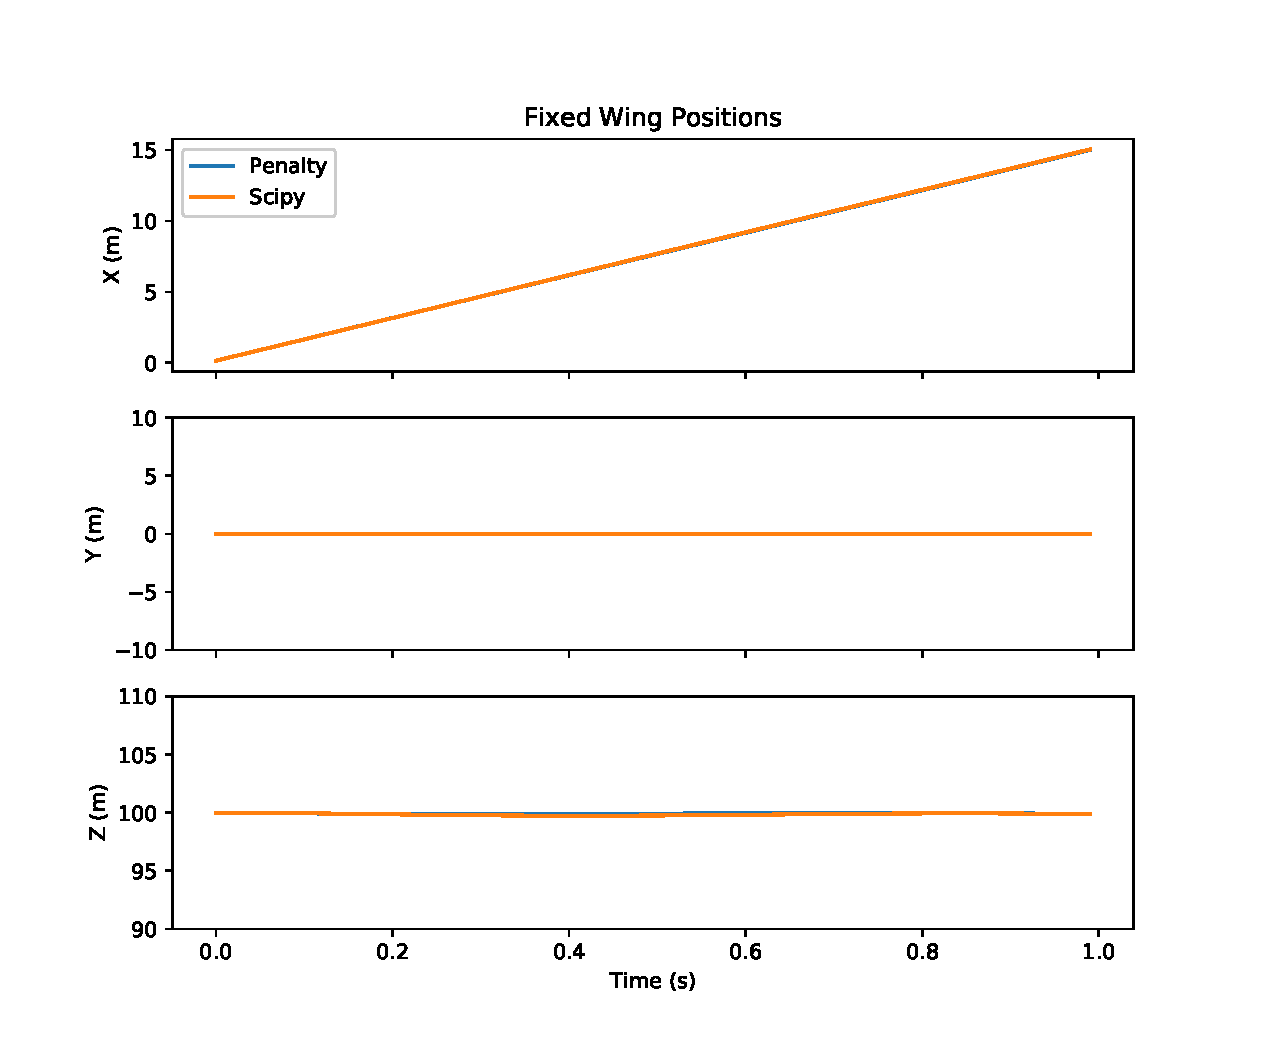
\includegraphics[width=0.45\textwidth]{figures/positions1_bc.eps}
		\label{fig:sub1}
	}
	\qquad
	\subfloat[]{
		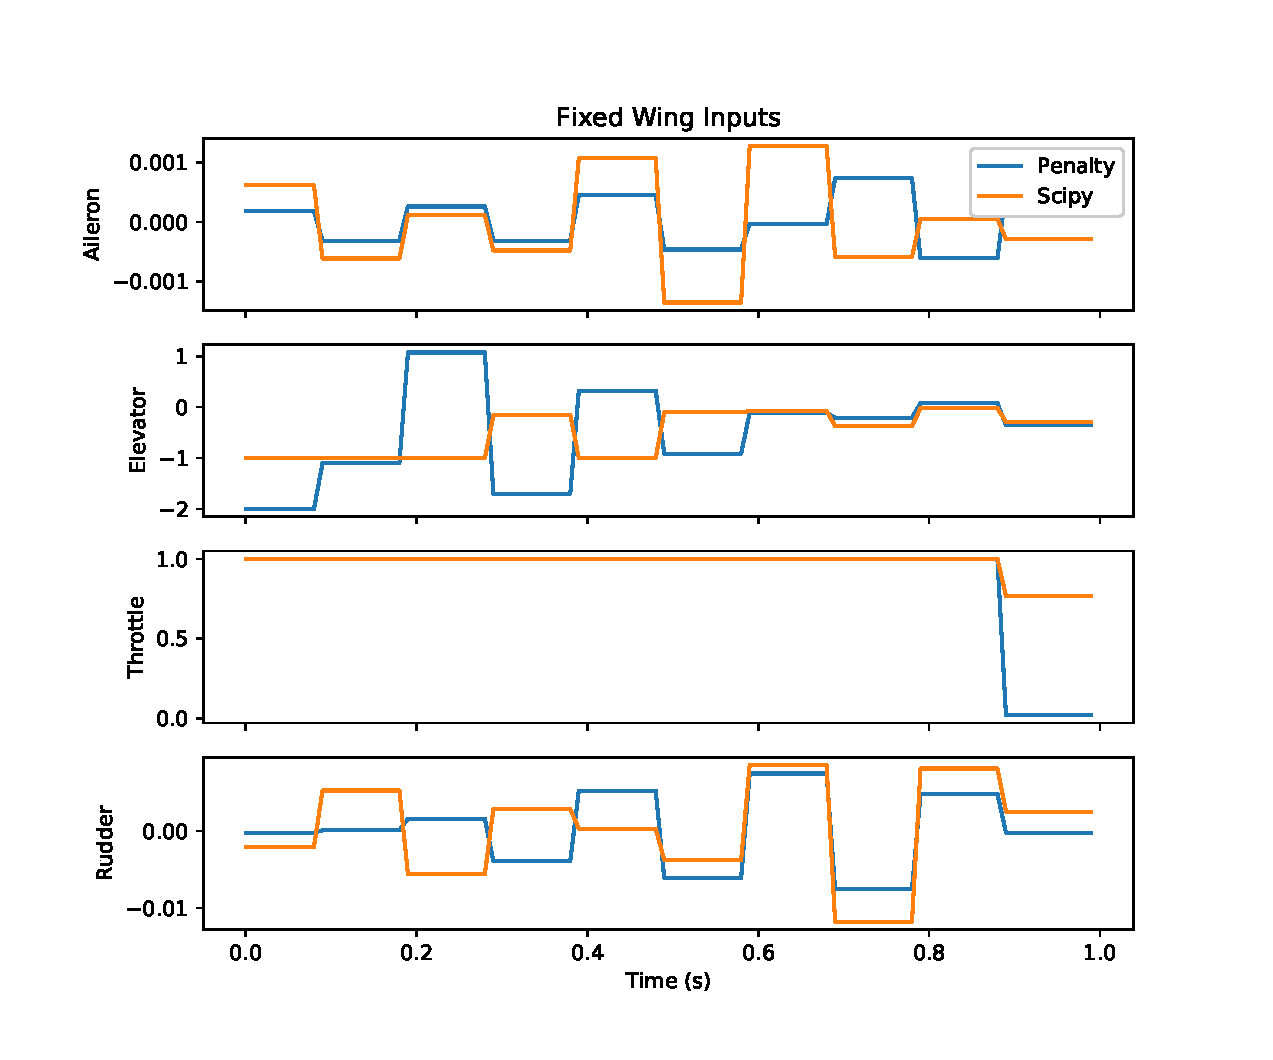
\includegraphics[width=0.45\textwidth]{figures/inputs_bc.eps}
		\label{fig:sub2}
	}
	\caption{label}
	\label{fig:bc}
\end{figure}


\begin{figure}[htbp]
	\centering
	\subfloat[]{
		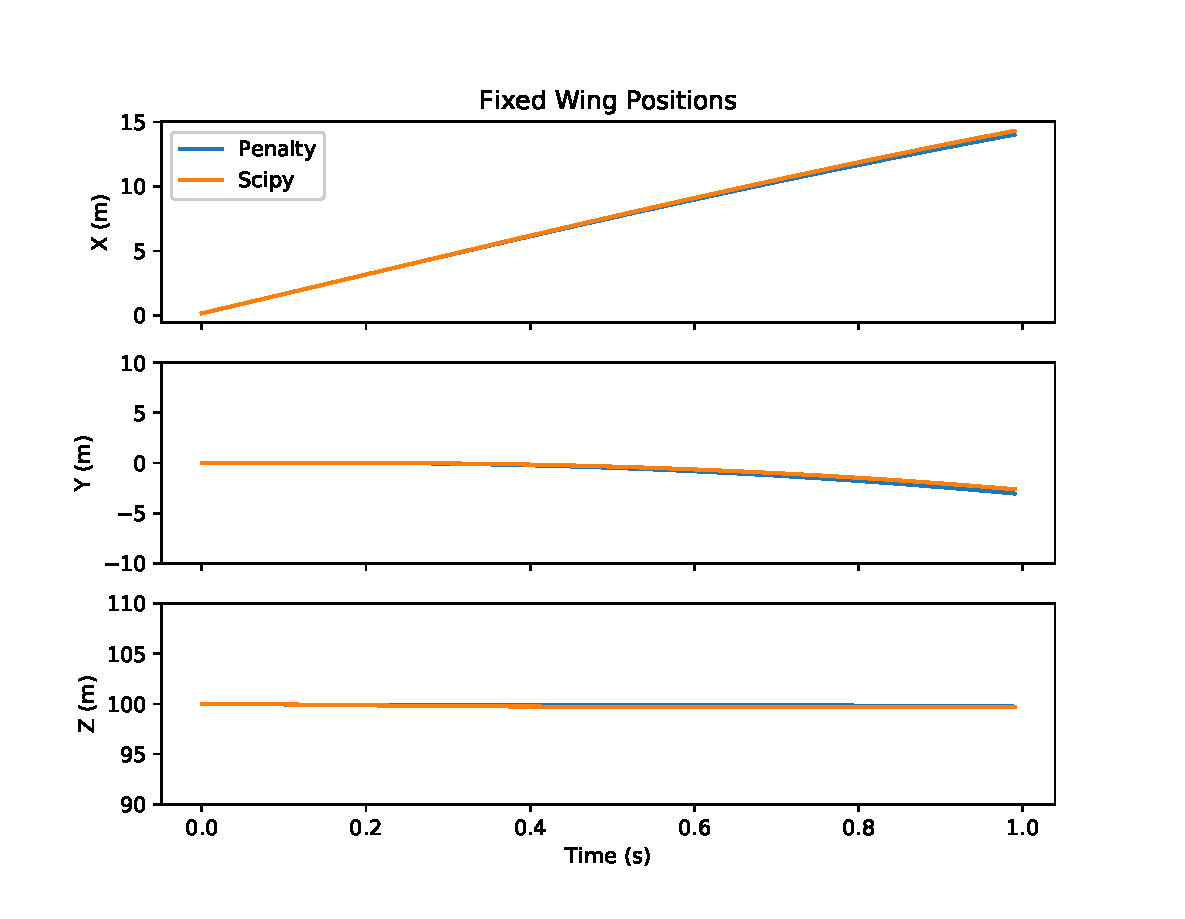
\includegraphics[width=0.45\textwidth]{figures/positions1.eps}
		\label{fig:sub1}
	}
	\qquad
	\subfloat[]{
		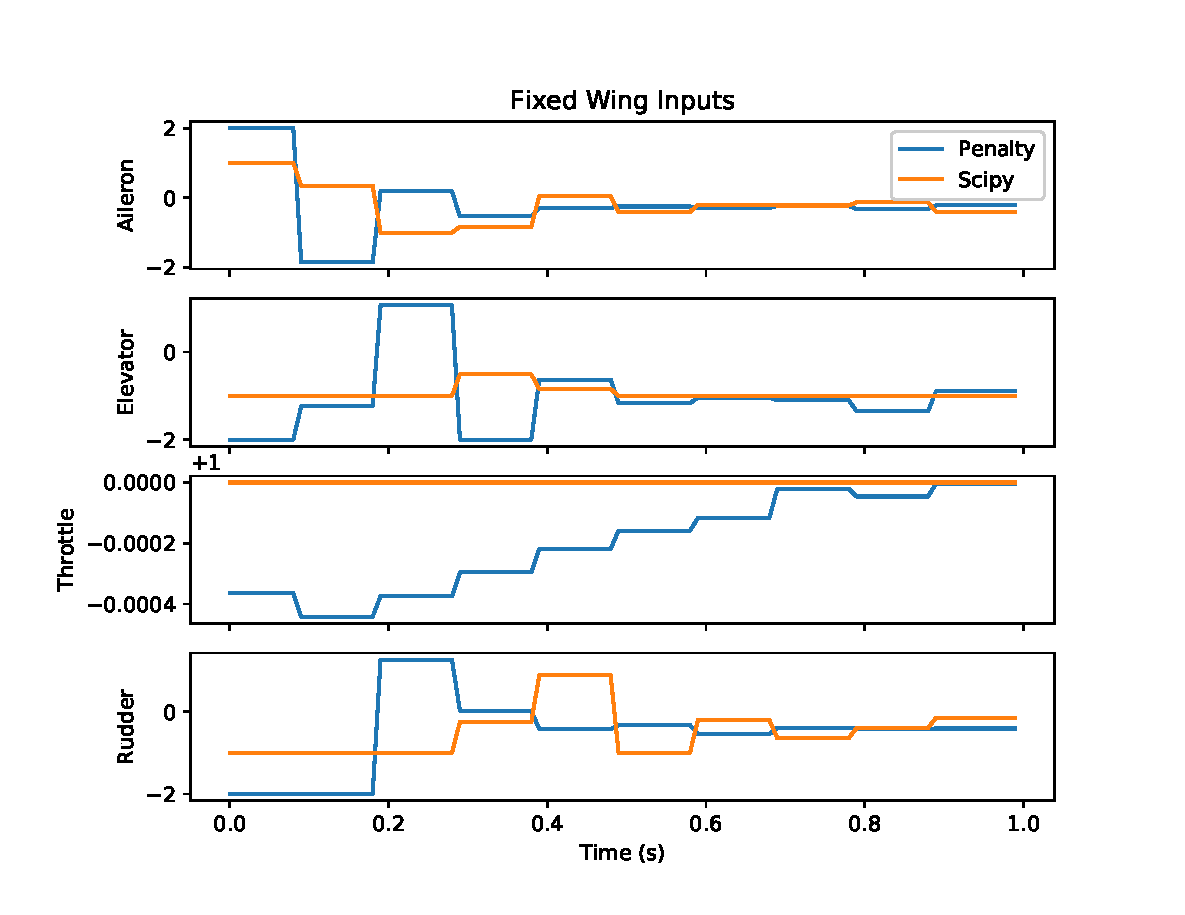
\includegraphics[width=0.45\textwidth]{figures/inputs.eps}
		\label{fig:sub2}
	}
	\caption{label}
	\label{fig:commanded_dir}
\end{figure}

\begin{figure}[htbp]
	\centering
	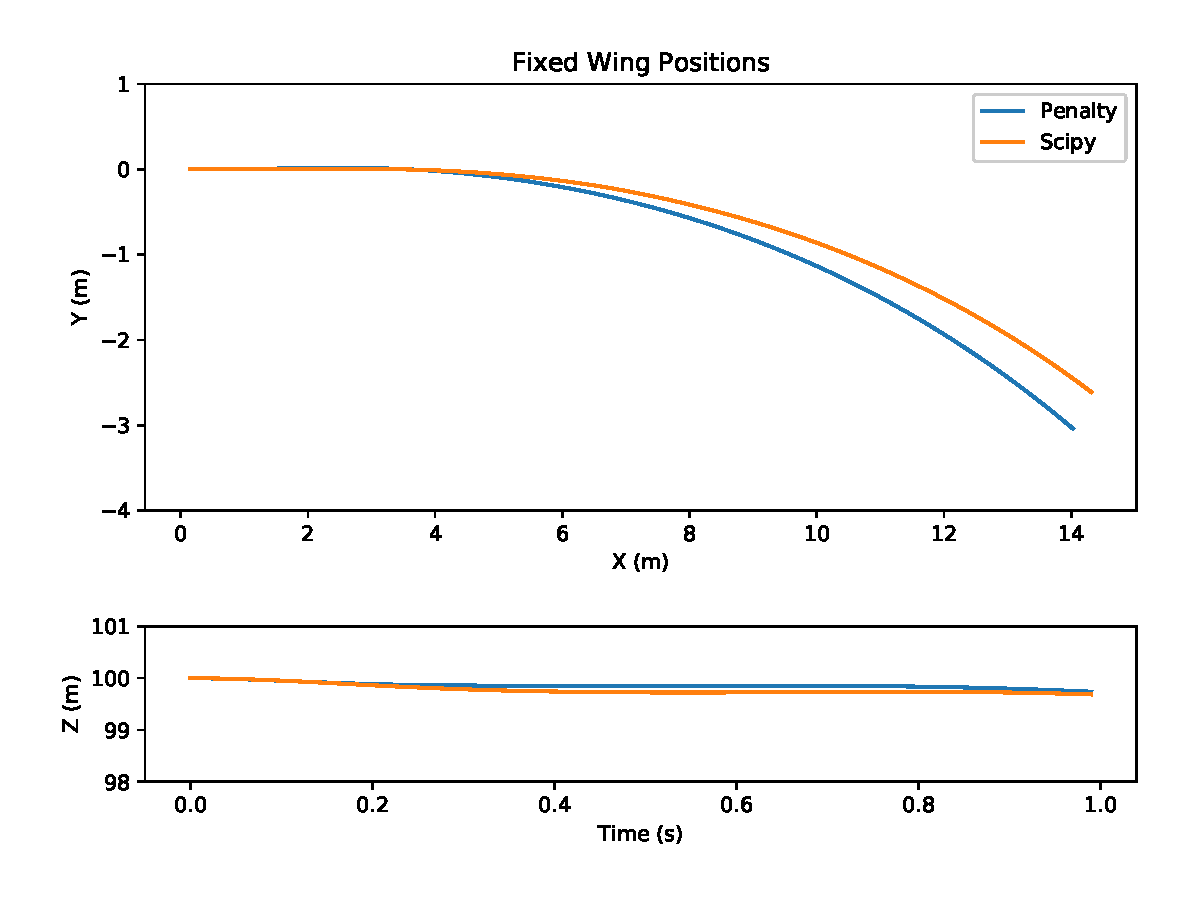
\includegraphics[width=0.45\textwidth]{figures/positions2.eps}
	\caption{label}
	\label{fig:commanded_dir2}
\end{figure}




\section*{Convergence}







\section*{Discussion}





\begin{appendices}
	
\section{Aircraft Dynamics}
\label{sec:dynamics}

The aircraft's position, velocity, attitude, and angular rate evolve in time according to
\begin{align}
\dot{\mathbf{p}}_{b/I}^{I} & =\left(R_{I}^{b}\right)^{\top}\mathbf{v}_{b/I}^{b}\label{eq:lqr_pdot_true}\\
\dot{\mathbf{v}}_{b/I}^{b} & =\frac{1}{m}\mathbf{f}^{b}-\boldsymbol{\omega}_{b/I}^{b}\times\mathbf{v}_{b/I}^{b}\label{eq:lqr_vdot_true}\\
\dot{\mathbf{q}}_{I}^{b} & =\boldsymbol{\omega}_{b/I}^{b}\label{eq:lqr_qdot_true}\\
\dot{\boldsymbol{\omega}}_{b/I}^{b} & =J^{-1}\left(\boldsymbol{\tau}^{b}-\boldsymbol{\omega}_{b/I}^{b}\times J\boldsymbol{\omega}_{b/I}^{b}\right),\label{eq:lqr_omegadot_true}
\end{align}
where $m$ is the aircraft's mass, $J$ is the aircraft's inertia matrix, and $\mathbf{f}^b$ and $\boldsymbol{\tau}^b$ are the force and torque applied to the aircraft body~\cite{beard2012small}.

We assume that the aircraft is equipped with the four control inputs: aileron, elevator, throttle, and rudder.
The aircraft receives a throttle signal $s_t\in\left[0,1\right]$ and signals for aileron, elevator, and rudder given by
\begin{align}
s_{a} &= \frac{\delta_{a}}{\delta_{a_{max}}}\in\left[-1,1\right] \\
s_{e} &= \frac{\delta_{e}}{\delta_{e_{max}}}\in\left[-1,1\right] \\
s_{r} &= \frac{\delta_{r}}{\delta_{r_{max}}}\in\left[-1,1\right],
\end{align}
where $\delta_*$ denotes deflection angle in radians and $\delta_{*_{max}}$ is the physically defined, maximum angle of deflection.

Vehicle air velocity, air speed, angle of attack, and side slip angle are defined by
\begin{align}
\mathbf{v}_{a/I}^{b} & =\mathbf{v}_{b/I}^{b}-R_{I}^{b}\mathbf{v}_{w/I}^{I}\\
V_{a} & =\norm{\mathbf{v}_{a/I}^{b}} \\
\alpha & =\tan^{-1}\left(\frac{\mathbf{e}_{3}^{\top}\mathbf{v}_{a/I}^{b}}{\mathbf{e}_{1}^{\top}\mathbf{v}_{a/I}^{b}}\right)\\
\beta & =\sin^{-1}\left(\frac{\mathbf{e}_{2}^{\top}\mathbf{v}_{a/I}^{b}}{V_{a}}\right),
\end{align}
where $\mathbf{v}_{w/I}^I$ is the wind velocity expressed in the inertial frame.

Nondimensionalized coefficients of lift and drag are defined by
\begin{align}
C_{L}\left(\alpha\right) & =\left(1-\sigma\left(\alpha\right)\right)\left[C_{L_{0}}+C_{L_{\alpha}}\alpha\right]+\sigma\left(\alpha\right)\left[2\mathrm{sign}\left(\alpha\right)\sin^{2}\alpha\cos\alpha\right]\nonumber\\
C_{D}\left(\alpha\right) & =C_{D_{p}}+\frac{S\left(C_{L_{0}}+C_{L_{\alpha}}\alpha\right)^{2}}{\pi eb^{2}},
\end{align}
where
\begin{equation}
\sigma\left(\alpha\right) =\frac{1+e^{-M\left(\alpha-\alpha_{0}\right)}+e^{M\left(\alpha+\alpha_{0}\right)}}{\left(1+e^{-M\left(\alpha-\alpha_{0}\right)}\right)\left(1+e^{M\left(\alpha+\alpha_{0}\right)}\right)}.
\end{equation}
Nondimensionalized coefficients of force in the body $x$ and $z$ axes are therefore given by
\begin{align}
C_{X}\left(\alpha\right) & =-C_{D}\left(\alpha\right)\cos\alpha+C_{L}\left(\alpha\right)\sin\alpha\\
C_{X_{q}}\left(\alpha\right) & =-C_{D_{q}}\cos\alpha+C_{L_{q}}\sin\alpha\\
C_{X_{\delta_{e}}}\left(\alpha\right) & =-C_{D_{\delta_{e}}}\cos\alpha+C_{L_{\delta_{e}}}\sin\alpha\\
C_{Z}\left(\alpha\right) & =-C_{D}\left(\alpha\right)\sin\alpha-C_{L}\left(\alpha\right)\cos\alpha\\
C_{Z_{q}}\left(\alpha\right) & =-C_{D_{q}}\sin\alpha-C_{L_{q}}\cos\alpha\\
C_{Z_{\delta_{e}}}\left(\alpha\right) & =-C_{D_{\delta_{e}}}\sin\alpha-C_{L_{\delta_{e}}}\cos\alpha.
\end{align}

Consequently, the force and torque expressed in the body frame are given by
\begin{align}
\mathbf{f}^{b} & =mR_{I}^{b}\mathbf{g}^{I}+\frac{\rho V_{a}^{2}S}{2}\bigg(C_{F}\left(\alpha,\beta\right)+\left.\frac{1}{2V_{a}}C_{F_{\omega}}\left(\alpha\right)\boldsymbol{\omega}_{b/I}^{b}+C_{F_{u}}\left(\alpha\right)\mathbf{u}\right)+\nonumber\\
&\quad\rho S_{prop}C_{prop}\mathbf{e}_{3}^{\top}\mathbf{u}\left(V_{a}+\mathbf{e}_{3}^{\top}\mathbf{u}\left(k_{motor}-V_{a}\right)\right)\cdot\nonumber\left(k_{motor}-V_{a}\right)\mathbf{e}_{1}\nonumber\\
\boldsymbol{\tau}^{b} & =\frac{\rho V_{a}^{2}S}{2}C_{bc}\bigg(C_{\tau}\left(\alpha,\beta\right)+\frac{1}{2V_{a}}C_{\tau_{\omega}}\boldsymbol{\omega}_{b/I}^{b}+ C_{\tau_{u}}\mathbf{u}\bigg)-k_{T_{p}}\left(k_{\Omega}\mathbf{e}_{3}^{\top}\mathbf{u}\right)^{2}\mathbf{e}_{1},\nonumber
\end{align}
where
\begin{align}
\mathbf{u} & =\begin{bmatrix}s_{a} & s_{e} & s_{t} & s_{r}\end{bmatrix}^{\top}\\
C_{F}\left(\alpha,\beta\right) & =\begin{bmatrix}C_{X}\left(\alpha\right)\\
C_{Y_{0}}+C_{Y_{\beta}}\beta\\
C_{Z}\left(\alpha\right)
\end{bmatrix}\\
C_{F_{\omega}}\left(\alpha\right) & =\begin{bmatrix}0 & C_{X_{q}}\left(\alpha\right)c & 0\\
C_{Y_{p}}b & 0 & C_{Y_{r}}b\\
0 & C_{Z_{q}}\left(\alpha\right)c & 0
\end{bmatrix}\\
C_{F_{u}}\left(\alpha\right) & =\begin{bmatrix}0 & C_{X_{\delta_{e}}}\left(\alpha\right)\delta_{e_{max}} & 0 & 0\\
C_{Y_{\delta_{a}}}\delta_{a_{max}} & 0 & 0 & C_{Y_{\delta_{r}}}\delta_{r_{max}}\\
0 & C_{Z_{\delta_{e}}}\left(\alpha\right)\delta_{e_{max}} & 0 & 0
\end{bmatrix}\\
C_{bc} & =\begin{bmatrix}b & 0 & 0\\
0 & c & 0\\
0 & 0 & b
\end{bmatrix}\\
C_{\tau}\left(\alpha,\beta\right) & =\begin{bmatrix}C_{l_{0}}+C_{l_{\beta}}\beta\\
C_{m_{0}}+C_{m_{\alpha}}\alpha\\
C_{n_{0}}+C_{n_{\beta}}\beta
\end{bmatrix}\\
C_{\tau_{\omega}} & =\begin{bmatrix}C_{l_{p}}b & 0 & C_{l_{r}}b\\
0 & C_{m_{q}}c & 0\\
C_{n_{p}}b & 0 & C_{n_{r}}b
\end{bmatrix}\\
C_{\tau_{u}} & =\begin{bmatrix}C_{l_{\delta_{a}}}\delta_{a_{max}} & 0 & 0 & C_{l_{\delta_{r}}}\delta_{r_{max}}\\
0 & C_{m_{\delta_{e}}}\delta_{e_{max}} & 0 & 0\\
C_{n_{\delta_{a}}}\delta_{a_{max}} & 0 & 0 & C_{n_{\delta_{r}}}\delta_{r_{max}}
\end{bmatrix}.
\end{align}
\end{appendices}

% This is for the bibliography.  Note that it is using sample.bib 
% you would need to provide your own bibtex file.

\bibliographystyle{unsrt}
\bibliography{references}




\end{document}